\section{Evaluation Scenarios, Results and Discussions}
\label{sec:evaluation:scenarios}

% divide the tests into two stages:
% 1) Test SA³ with fully simulated conditions -> use the IS'14 paper to extract the scenarios but run them agian, since now location infrence is used. Use activity-based evaluation and argue that this evaluation is important to assess the performance of the clustering initialisation. If the initialisation is bad activity-wise, the next steps will not perform well.
% 2) Test the full EAM learning system in two steps: activity clustering (SA³ + AA -> use action-based evaluation) and the full system (activity clustering + AML -> use model-based evaluation). Use Expert Systems with Applications paper to extract evaluation scenarios, metrics and results.

% In all the cases, explain why we are running such experiments and what we are trying to validate with them. 

Using the tools and methodologies described in Section \ref{sec:evaluation:methodology}, several evaluation scenarios have been prepared to test and validate the most important aspects of the EAM learning system. More concretely, three major evaluation scenarios can be distinguished:

\begin{enumerate}
 \item $SA^3$ evaluation scenarios: $SA^3$ is a very important part of the whole EAM learning system, since it is the initialisation step of the clustering algorithm. The performance of $SA^3$ has to be carefully analysed to understand how it works, its main advantages and strong points as well as its main weaknesses. Remember that $AA$ algorithm works on the results of $SA^3$, adding -or not- actions to the initial action clusters detected by $SA^3$. But if $SA^3$ fails at detecting an activity, $AA$ cannot recover it. Thus, the performance of $SA^3$ in all possible situations is key for the performance of the clustering process and in consequence, the performance of the EAM learning system.
 \item Activity clustering evaluation scenarios: the activity clustering process is the sum of the $SA^3$ and $AA$ algorithms. As a result of the process itself, every sensor activation of a dataset is labelled and several clusters for the defined activities are obtained. Action clusters' quality is directly linked to labelling performance. Remember that those action clusters are finally processed by the $AML$ algorithm to learn extended activity models, so assessing the performance of the clustering process by means of labelled sensor activations is very important.
 \item EAM learning evaluation scenarios: finally, the EAM learning system has to be evaluated. The system is composed by the sequential use of $SA^3$, $AA$ and $AML$. Evaluation scenarios have to be set-up in order to validate that the EAM learning system is able to learn extended activity models for different users. The results obtained in those evaluation scenarios are the most important ones, because they give a clear vision of the performance of the whole system.
\end{enumerate}

\subsection{$SA^3$ performance}
\label{subsec:evaluation:sa3}

\subsubsection{Evaluation scenarios and metrics}
\label{subsubsec:evaluation:sa3:scenarios}
To assess the performance of $SA^3$ exhaustively, the features of the synthetic dataset generator will be used to set up different kinds of scenarios. To prepare those scenarios, surveys will not be used. In the case of $SA³$, the main interest is to measure the performance in presence of increasing noise, activities with several variations, varied order of actions, using IAMs that share the same actions, activity sequences that are very close in time, etc. As $SA^3$ alone is not going to be used for real applications, the usage of surveys is not necessary. $SA^3$ makes sense inside the complete activity clustering algorithm, whose performance will be tested using real users' inputs.

With this purpose, four scenarios have been prepared: 

\begin{enumerate}
 \item The ideal scenario: $SA³$ will be tested in ideal conditions, i.e. there is no sensor noise in the dataset.
 \item Missing sensor noise scenario: increasing missing error probability is introduced to two sensors that are mapped to actions of the IAMs of two activities, to understand how the detection of those activities evolves compared to noiseless activities. It is also important to see whether the missing noise affecting to some activities influence the detection of the others.
 \item Positive sensor noise scenario: increasing positive noise is introduced to assess the performance of $SA³$ in presence of positive noise.
 \item Demanding activities scenario: the fourth scenario tests how $SA³$ performs when IAMs of several activities share many actions among them. 
\end{enumerate}

\begin{figure}
\begin{small}
\lstset{linewidth=\textwidth}
\begin{lstlisting}
MakeCoffee 2
0.5 mugSens@0 smilkSens@20 microwaveSens@20 afcoffeeSens@120 
    wsugarSens@20
0.5 cupSens@0 ktapSens@10 microwaveSens@15 wsugarSens@90 
    afcoffeeSens@30
MakeChocolate 2
0.8 mugSens@0 wmilkSens@20 microwaveSens@20 chocoSens@120
0.2 cookerSens@0 potSens@5 wmilkSens@20 chocoSens@30 
    mugSens@200
MakePasta 2
0.8 potSens@0 ktapSens@20 cookerSens@30 macaroniSens@120 
    ftomatoSens@600
0.2 spaghettiSens@0 potSens@20 ktapSens@25 cookerSens@30 
    baconSens@50 creamSens@600
BrushTeeth 2
0.7 brusherSens@0 toothpasteSens@5 glassSens@30 btapSens@5
0.3 brusherSens@0 toothpasteSens@5 glassSens@30 btapSens@5 
    dentalflossSens@15
WatchTelevision 2
0.5 sofaSens@0 rcontrolSens@5 tvSens@10
0.5 rcontrolSens@0 tvSens@5 sofaSens@5
WashHands 2
0.85 btapSens@0 bsoapSens@15 handcreamSens@40
0.15 btapSens@0 bsoapSens@15
ReadBook 2
0.9 bookbSens@0 bedSens@10 blampSens@5
0.1 bookaSens@0 sofaSens@10
\end{lstlisting}
\end{small}
\caption{Sensor activation patterns for the defined activities.}
\label{fig:basic-script-activities}
\end{figure}

The base of the first three scenarios is an ADL script prepared to offer some common features to all experiments. From the activity models point of view: (i) several variations for every activity, (ii) different probability distributions between activity variations, (iii) varied order of actions in activities and (iv) varied time lapses between consecutive sensor activations. From the behaviour model perspective: (i) different day types, (ii) activities which are very close in time and (iii) combinations of sequences and alterations.

The prepared ADL script reflects all those features and tries to be realistic in the definition of the activity and behaviour models. However, notice that at this point, realism is not important (the following evaluation scenarios will address realism properly). Figure \ref{fig:basic-script-activities} shows the defined seven activities of daily living with all the sensor activation patterns and occurrence probabilities. As it can be seen in the Figure, defined activities are: MakeCoffee, MakeChocolate, MakePasta, BrushTeeth, WatchTelevision, WashHands and ReadBook. Different probability distributions can be found for different activities. For example, MakeCoffee has an even occurrence probability for its two variations (50\% - 50\%). However, ReadBook is very unbalanced (90\% - 10\%). Varied order of actions and time lapses can also be seen in the sensor activation patterns of each activity. Finally, some activities contain a lot of sensor activations - six in the case of MakePasta - whereas some others are very short - WashHands or ReadBook with only two -. In general, activity models reflect all the desired features to test the performance of $SA³$, as identified in the paragraph above.

\begin{figure}
\begin{small}
\lstset{linewidth=\textwidth}
\begin{lstlisting}
Prob 0.43 4
S 7:00-7:30 MakeChocolate@0 BrushTeeth@120 WashHands@30
S 13:00-13:30 MakePasta@0 MakeCoffee@60 BrushTeeth@1800
S 20:00-20:30 MakePasta@0 BrushTeeth@200 ReadBook@150
A 18:00-19:30 WatchTelevision 0.8
Prob 0.28 2
S 7:00-7:30 MakeChocolate@0 BrushTeeth@100 WashHands@30
S 20:30-21:00 BrushTeeth@0 ReadBook@50
Prob 0.29 5
S 9:00-10:00 MakeChocolate@0 WatchTelevision@30 BrushTeeth@1800
S 13:30-14:30 MakePasta@0 BrushTeeth@150
S 22:00-23:00 BrushTeeth@0 WashHands@10
A 15:00-16:00 WatchTelevision 0.75
A 18:00-20:00 ReadBook 0.5
\end{lstlisting}
\end{small}
\caption{Behaviour models for a given user.}
\label{fig:basic-script-behaviour}
\end{figure}

Behaviour models defined for the first three evaluation scenarios are depicted in Figure \ref{fig:basic-script-behaviour}. Three typical days are defined with different occurrence probabilities. The first one has three sequences and one alteration. Activity WashHands is very close in time to activity BrushTeeth, for example. The second day type tries to simulate a typical day where the inhabitant spends few time in home, showing a big time difference between both activity sequences. Finally, the third day type contains two alterations and three new activity sequences where some activities are again very close in time.

Another common element of the first three evaluation scenarios is the IAMs of the activities. All seven activities have the same IAMs alongside the three scenarios. Figure \ref{fig:basic-iams} shows the IAMs used for the experiments. It is very important to keep the same IAMs in all the experiments, since IAMs aim at describing incomplete but generic activity models for any user.

\begin{figure}
\begin{small}
\lstset{linewidth=\textwidth}
\begin{lstlisting}
   "MakeCoffee": {
      "type": ["Cooking"],
      "location": ["Kitchen"],
      "IAM": ["hasContainer", "hasCoffee"],
      "duration": 360
   },
   "MakeChocolate": {
      "type": ["Cooking"],
      "location": ["Kitchen"],
      "IAM": ["hasContainer", "hasChocolate"],
      "duration": 500
   },
   "MakePasta": {
      "type": ["Cooking"],
      "location": ["Kitchen"],
      "IAM": ["hasPasta", "useCookingAppliance", 
              "useCookingUtensil"],
      "duration": 1200
   },
   "BrushTeeth": {
      "type": ["Hygiene"],
      "location": ["Bathroom"],
      "IAM": ["hasBrusher", "hasToothpaste", "turnOnTap"],
      "duration": 130
   },
   "WatchTelevision": {
      "type": ["Entertainment"],
      "location": ["Lounge"],
      "IAM": ["hasRemoteControl", "useTV"],
      "duration": 40
   },
   "WashHands": {
      "type": ["Hygiene"],
      "location": ["Bathroom"],
      "IAM": ["turnOnTap", "hasSoap"],
      "duration": 90
   },
   "ReadBook": {
      "type": ["Entertainment"],
      "location": ["Bedroom", "Lounge"],
      "IAM": ["hasBook", "useFurniture"],
      "duration": 30
   } 
\end{lstlisting}
\end{small}
\caption{The IAMs of all seven defined activities for the first three evaluation scenarios.}
\label{fig:basic-iams}
\end{figure}

The fourth evaluation scenario is different from the other three scenarios. The idea is to use some activities whose IAMs share the same actions. For that purpose, and trying to keep the realism, the following seven activities have been defined: MakeCoffee, MakeWhippedCream, MakeTiramisu, BrushTeeth, WatchTelevision, WashHands and ReadBook. The first three activities' IAMs are formed by the same four actions. More concretely:

\begin{small}
\lstset{linewidth=\textwidth}
\begin{lstlisting}
 IAM(MakeCoffee) = {hasContainer, hasCoffee, hasFlavour}
 IAM(MakeWhippedCream) = {hasContainer, hasCream, hasFlavour}
 IAM(MakeTiramisu) = {hasContainer, hasCream, hasCoffee} 
\end{lstlisting}
\end{small}

The other activities are defined as in the previous scenarios. So the aim of this evaluation scenario is to see how $SA³$ behaves with challenging IAMs. To focus only on the pattern recognition performance, no noise is added to this fourth evaluation scenario.

For all four evaluation scenarios the same metrics have been used. The most important aspect for $SA³$ to be evaluated is whether activities are well detected. So labels given to sensor activations are not important. Rather, a comparison between the start and end times of the activity detected by $SA³$ and the real activity has to be done. Assume $A_R$ is the real activity and $A_{SA³}$ the activity detected by $SA³$. $A_{SA³}$ is a correct activity detection if $A_R$ contains $A_{SA³}$ and both activities have the same label:

\begin{equation}
\begin{gathered}
 t_{start}(A_R) \leq t_{start}(A_{SA³}) \mbox{ and } t_{end}(A_{SA³}) \leq t_{end}(A_R) \\
 Label(A_R) = Label(A_{SA³})
\end{gathered}
\label{metric-sa3}
\end{equation}

This evaluation criterion is called \textit{activity-based evaluation}. Using activity-based evaluation criterion, true positives, false positives and false negatives are calculated for every activity, comparing the output of $SA³$ with the ground truth.

\subsubsection{Results}
\label{subsubsec:evaluation:sa3:results}
% Put the tables and graphics here

\paragraph*{Ideal scenario}

To test the performance of $SA^3$ and have a base reference, the ideal scenario has been designed. The ADL script has already been described (Section \ref{subsubsec:evaluation:sa3:scenarios}) and it contains varying order of sensor activations per activity, varied occurrence probability distributions and varied time lapses between sensor activations and activities. The aim of the ideal scenario is to obtain a base reference of the performance of $SA³$ in noiseless conditions. Activity-based evaluation is used and true positives, false positives and false negatives are measured. 

With the objective of getting reliable results, 130 days have been simulated. More concretely, the sensor activation dataset contains 4093 sensor activations describing a total number of 1027 activity instances. The results are shown in Table \ref{tab-sa3-ideal}. For each activity, the number of instances and the percentages of true positives, false positives and false negatives are given.

\begin{table}[htbp]\scriptsize
  \begin{center}
        \begin{tabular}{ccccc}
            \hline            
            \textbf{Activity} & \textbf{Instances} & \textbf{True Positives (\%)} &  \textbf{False Positives (\%)} & \textbf{False Negatives (\%)}\\             
            \hline
            MakeChocolate   & 130 & 100 & 0 & 0 \\
	    WatchTelevision & 103 & 100 & 0 & 0 \\
	    BrushTeeth      & 350 & 100 & 0 & 0 \\
	    WashHands       & 130 & 100 & 0 & 0 \\
	    MakePasta       & 146 & 100 & 0 & 0 \\
	    ReadBook        & 112 & 100 & 0 & 0 \\
	    MakeCoffee      & 56 & 100 & 0 & 0 \\
            \hline
        \end{tabular}                
        \caption{Results of the $SA³$ algorithm for the ideal scenario.}
        \label{tab-sa3-ideal}
    \end{center}
\end{table}

Table \ref{tab-sa3-ideal} shows that the 100\% of all activities are properly captured by $SA³$ under ideal conditions. There are neither false positives nor false negatives. Remember that activity-based evaluation does not check for the labels of every sensor activation. The fact that a 100\% of all activities are properly captured indicates that $SA³$ gets activity time locations robustly.

\paragraph*{Sensor missing noise scenario}

For the next experiments, assessing the performance of $SA³$ under sensor missing error noise is the objective. In principle, the completion criterion of the activity sequence finding step of $SA^3$ suggests that if a sensor activation which is mapped to one of the IAMs fails, $SA³$ would fail to detect that activity (see Section \ref{subsec:clustering:sa3:find} for a detailed explanation). In order to test that suggestion, two of the seven activities have been chosen. Sensor activations which are mapped to the IAMs of those activities are given an increasing missing probability, to see how this missing noise affects the detection of those activities. The rest of the activities are kept noiseless, to measure the effect of missing noise in other activities. Table \ref{tab-sa3-missing} shows the results for the sensor missing noise scenario. The activities which suffer missing noise are marked with an asterisk (MakeChocolate and BrushTeeth). Five experiments are run, each of them simulating 130 days. Sensor missing probabilities are 0.01, 0.02, 0.05, 0.07 and 0.1. For each experiment, true positives, false positives and false negatives are measured, using the activity-based evaluation criterion. 

\begin{table}[htbp]\scriptsize
  \begin{center}
        \begin{tabular}{cccccc}
            \hline            
            \textbf{Activity} & \multicolumn{5}{c}{\textbf{Sensor missing probability}}\\
             & 0.01 & 0.02 & 0.05 & 0.07 & 0.1 \\
             & TP- FP - FN (\%) & TP - FP - FN (\%) & TP - FP - FN (\%) & TP - FP - FN (\%) & TP - FP - FN (\%)\\
            \hline
            MakeChocolate*   & 99.2 - 0 - 0.8 & 99.2 - 0 - 0.8 & 94.6 - 0 - 5.4 & 92.3 - 0 - 7.7 & 89.2 - 0 - 10.8 \\
	    WatchTelevision  & 100 - 0 - 0 & 100 - 0 - 0 & 100 - 0 - 0 & 100 - 0 - 0 & 100 - 0 - 0 \\
	    BrushTeeth*      & 98.9 - 0 - 1.1 & 98.6 - 0 - 1.4 & 96 - 0 - 4 & 93.8 - 0 - 6.2 & 89.4 - 0 - 10.6 \\
	    WashHands        & 100 - 0 - 0 & 100 - 0 - 0 & 100 - 0 - 0 & 100 - 0 - 0 & 100 - 0 - 0 \\
	    MakePasta        & 100 - 0 - 0 & 100 - 0 - 0 & 100 - 0 - 0 & 100 - 0 - 0 & 100 - 0 - 0 \\
	    ReadBook         & 100 - 0 - 0 & 100 - 0 - 0 & 100 - 0 - 0 & 100 - 0 - 0 & 100 - 0 - 0 \\
	    MakeCoffee       & 100 - 0 - 0 & 100 - 0 - 0 & 100 - 0 - 0 & 100 - 0 - 0 & 100 - 0 - 0 \\
            \hline
        \end{tabular}                
        \caption{Results of $SA³$ for the sensor missing noise scenario, where TP: true positives, FP: false positives and FN: false negatives. The activities affected by the noise have an asterisk.}
        \label{tab-sa3-missing}
    \end{center}
\end{table}

As it can be seen in Table \ref{tab-sa3-missing}, the performance of $SA³$ for the rest of activities does not vary. It keeps on producing 100\% of true positives, while false positives and negatives are null. However, true positive rate of activities MakeChocolate and BrushTeeth seems to be linearly reducing with sensor missing noise probability. The reduction of true positives generates the appearance of false negatives, since those activities that are not detected, are labelled as None. Thus, they are considered false negatives. There is no effect in false positives, but the effect on true positives is clear, as expected. To make the linearity more clear, Figure \ref{fig:sa3-missing} plots true positive rates for both activities for measured sensor missing noise probabilities. 

\begin{figure}[htbp]
\centering
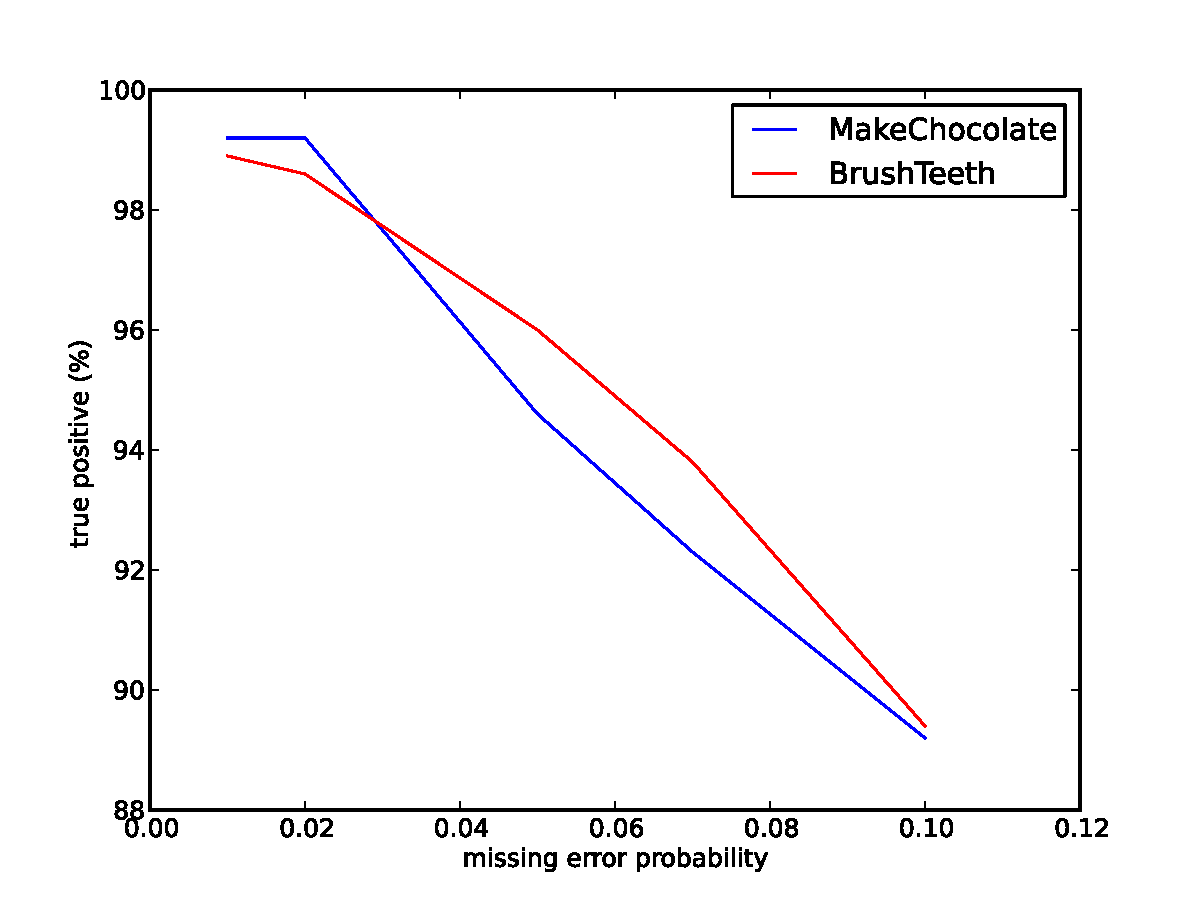
\includegraphics[width=10cm]{missing_error_graphic.pdf}
    \caption{The true positive percentages of $SA^3$ for activities MakeChocolate and BrushTeeth in presence of increasing sensor missing noise.}
    \label{fig:sa3-missing}
\end{figure}

Taking into account that noise generation is probabilistically accomplished in the synthetic dataset generator, Figure \ref{fig:sa3-missing} is a confirmation of the inverse linear relation between sensor missing noise and $SA³$ activity detection performance. When missing error increases, activity detection decreases. 

\paragraph*{Sensor positive noise scenario}

To test the sensor positive noise scenario, five experiments have been run. For each of the experiments, six sensors are picked up randomly and they are assigned increasing sensor positive noise probabilities. This strategy allows measuring the performance of $SA³$ in presence of positive noise. For each of the experiments 130 days are simulated again. To have a reference of the level of noise, sensor activations in each dataset scale from 5054 to 8850. The noiseless scenario presented 4093 sensor activations, so the noisiest dataset contains around 46\% more sensor activations. Table \ref{tab-sa3-positive} shows the results for the sensor positive noise scenario. Each experiment is identified by its noise level, where 0.05 means that all randomly selected sensors have a positive noise probability of 0.05 per hour. For each experiment, true positives, false positives and false negatives are depicted.

\begin{table}[htbp]\scriptsize
    \begin{center}    
        \begin{tabular}{cccccc}
            \hline            
            \textbf{Activity} & \multicolumn{5}{c}{\textbf{Sensor positive probability}}\\
             & 0.05 & 0.1 & 0.15 & 0.2 & 0.25 \\
             & TP - FP - FN (\%) & TP - FP - FN (\%) & TP - FP - FN (\%) & TP - FP - FN (\%) & TP - FP - FN (\%)\\
            \hline
            MakeChocolate   & 100 - 0 - 0 & 100 - 0 - 0 & 100 - 0 - 0     & 100 - 0 - 0 & 100 - 0 - 0 \\
	    WatchTelevision & 100 - 0 - 0 & 100 - 0 - 0 & 99.1 - 0.9 - 0  & 100 - 0 - 0 & 100 - 0 - 0 \\
	    BrushTeeth      & 100 - 0 - 0 & 100 - 0 - 0 & 100 - 0 - 0     & 100 - 0 - 0 & 100 - 0 - 0 \\
	    WashHands       & 100 - 0 - 0 & 100 - 0 - 0 & 100 - 0 - 0     & 100 - 0 - 0 & 100 - 0 - 0 \\
	    MakePasta       & 100 - 0 - 0 & 100 - 0 - 0 & 100 - 0 - 0     & 100 - 0 - 0 & 99.3 - 0.7 - 0 \\
	    ReadBook        & 100 - 0 - 0 & 100 - 0 - 0 & 97.5 - 2.5 - 0  & 100 - 0 - 0 & 98.1 - 1.9 - 0 \\
	    MakeCoffee      & 100 - 0 - 0 & 100 - 0 - 0 & 100 - 0 - 0     & 100 - 0 - 0 & 100 - 0 - 0 \\
            \hline
        \end{tabular}          
        \caption{Results of $SA³$ for positive sensor noise scenario; TP: true positives; FP: false positives; FN: false negatives}
        \label{tab-sa3-positive}
    \end{center}
\end{table}

Table \ref{tab-sa3-positive} shows that sensor positive noise affects true positives and false positives. For the first one, a slight reduction for some activities can be seen. For the second one, some activities show rates that even being greater than zero, they are still very low, 2.5\% being the highest for those experiments. Exploring obtained data deeper, it was found that in some cases, the false positives are generated overlapped with the real activity, i.e. a false sensor activation appears close to the real activity and changes the real time assignments for that activity. This happens when a sensor activation which is mapped to an action in the IAM of a given activity is generated by chance very close in time from a real execution of that activity. The effect is that the $SA^3$ fails at annotating all real occurrences of a given activity and produces false positive annotations. This can be seen in activities WatchTelevision and MakePasta, for example. In some other cases, false positives do not affect the annotation of correct activities (look at ReadBook for 0.15 and 0.25 noise levels, where all instances of the activity were perfectly annotated). In those cases, the problem is that the IAM of activity ReadBook is composed by two actions: \textit{hasBook} and \textit{useFurniture}. As sensor activations for two sensors monitoring furniture and books were chosen randomly for noise generation, it turned out that both activations were given in such circumstances that they were detected as activities. However, they do not affect any other activity detection.

\paragraph*{Demanding activities scenario}

The final scenario aims at testing $SA³$ under demanding activities. As it has been explained in Section \ref{subsubsec:evaluation:sa3:scenarios}, demanding activities are those which share many common actions in their IAMs. It can be thought that as $SA³$ uses a pattern recognition algorithm where some specific domain-based criteria are applied, its performance could be affected by very similar IAMs. Those conditions are simulated using seven activities, where MakeCoffee, MakeTiramisu and MakeWhippedCream share the same four actions in their IAMs. Remember that even being very similar, they are still different and unique. For this special scenario, a total number of 1262 activity instances have been produced. No sensor noise has been produced for the experiment, since the objective is to see the effect of demanding activities. Obtained results can be seen in Table \ref{tab-sa3-demanding}.

\begin{table}[htbp]\scriptsize
    \begin{center}         
        \begin{tabular}{ccccc}
            \hline
            \textbf{Activity} & \textbf{Instances} & \textbf{True positives (\%)} & \textbf{False positives (\%)} & \textbf{False negatives (\%)} \\
            \hline
            MakeCoffee         & 222 & 100 & 0 & 0 \\
	    MakeTiramisu       & 120 & 100 & 0 & 0 \\
	    MakeWhippedCream   & 72  & 100 & 0 & 0 \\
	    WashHands          & 150 & 100 & 0 & 0 \\
	    BrushTeeth         & 420 & 100 & 0 & 0 \\
	    ReadBook           & 127 & 100 & 0 & 0 \\
	    WatchTelevision    & 151 & 100 & 0 & 0 \\
            \hline
        \end{tabular}  
        \caption{Results of $SA³$ for demanding activity models scenario.}
        \label{tab-sa3-demanding}
    \end{center}
\end{table}

Results show that $SA³$ is not affected by the similarity of IAMs, as long as they are unique. True positives are 100\% for all activities, whereas false positives and negatives are zero. The situation is exactly the same as in the ideal scenario. Notice that assuming unique IAMs for each activity is very reasonable, since if there are two equal IAMs for two activities, those two activities should actually be one. 

\subsubsection{Discussion about SA³}
\label{subsubsec:evaluation:sa3:discussion}

Results shown in Section \ref{subsubsec:evaluation:sa3:results} show that $SA^3$ can handle varying order of actions in activity performance without any problem. All four set-ups contain different activation patterns, where actions are executed in different orders. This can be seen in Figure \ref{fig:basic-script-activities}: every activity has different sensor activation sequences with varying orders. As the ideal scenario shows (Table \ref{tab-sa3-ideal}), the success rate of the algorithm for every activity is 100\% and neither false positives nor negatives are observed. Notice that sensor activation sequences used for each activity contain many actions which are not used to define any of the IAMs, but the algorithm still performs perfectly when detecting activities. Hence, $SA^3$ can also handle non-considered actions.

As far as noisy scenarios regard, results suggest that missing sensor activations cannot be properly handled by the algorithm, when those activations are linked to actions that are used to define IAMs, i.e. if a sensor activation which is mapped to one of the actions used to define the IAM of a concrete activity fails, that activity cannot be detected by $SA³$. The non-captured activities are proportional to the missing activation probability of those actions, as shown in Figure \ref{fig:sa3-missing}. This is due to the completeness criterion used in the second step of $SA^3$, as explained in Section \ref{sec:clustering:sa3}, which demands the presence of all actions in the IAM of an activity to consider an action sequence a valid activity. However, missing sensor noise only affects true positive and false negative rates of the activities which are faultily registered by sensors. False positive rates keep behaving as the ideal scenario. Moreover, a non-detection of an activity does not have any other effect on the other activities. Following this reasoning, a good way to minimise the impact of sensor missing noise is to monitor key objects for IAMs using robust sensors such as contact sensors.  

Independently from such robust monitoring strategies, it is reasonable to think whether algorithmic solutions to mitigate sensor missing noise can be adopted. The completion criterion is very restrictive in that sense, but it is also very reasonable, since if not, distinguishing real activity executions from positive noise would be very difficult, specially considering the low number of actions used in the IAMs (see Table \ref{tab-avg-actions-comp-t2}). Further approaches have not been analysed in this dissertation, because the low level of missing sensor noise in real environments makes the detection rates very good. However, some ideas are suggested in Chapter \ref{cha:conclusions} for their future development.

For sensor positive noise, the scenario is different. $SA^3$ has shown to perform reliably even with high levels of noise. For example, even having certain sensors with faulty activation probabilities of 0.25 per hour, average true positive rate over all activities is 99.9\%. Simultaneously, false positive rates are still very low, concretely 0.3\% in average, while false negative rates are 0. False positive activity detections are due to random occurrences of actions in time instants which make them compatible with the duration criterion of an activity. The probability of having such false positives increases as the noise level increases and the number of actions in IAMs decreases. However, the results obtained with the highest level of noise of the experiments show how robust $SA³$ is in such scenarios.

Finally, a test involving challenging activity models shown that as far as activity models are unique, $SA^3$ does not have any problem detecting them. Average true positive rate for all activities is 100\% and false positive and negative rates are 0, as it can be seen in Table \ref{tab-sa3-demanding}. Remember that the experiments for challenging or demanding activity models were performed without any noise. So results suggest that the performance is exactly the same as for the ideal scenario. 

In conclusion, $SA³$ has been tested for all the desired requirements listed in Section \ref{subsubsec:evaluation:sa3:scenarios}. From the activity models point of view: (i) several variations for every activity, (ii) different probability distributions between activity variations, (iii) varied order of actions in activities and (iv) varied time lapses between consecutive sensor activations. From the behaviour model perspective: (i) different day types, (ii) activities which are very close in time and (iii) combinations of sequences and alterations. All those features were present in all four evaluation scenarios, where ideal conditions, noisy scenarios and demanding activity models were also tested. Results suggest that $SA³$ is a very reliable tool to detect activity executions. It does not correctly label all the sensor activations, but it accurately captures activity time locations. Thus, it can be concluded that $SA³$ serves as a initialisation step for an activity clustering process.

\subsection{Activity clustering performance}
\label{subsec:evaluation:clustering}

\subsubsection{Evaluation scenarios and metrics}
\label{subsubsec:evaluation:clustering:scenarios}
Testing the activity clustering algorithm, i.e. $SA³ + AA$, requires the usage of the hybrid evaluation methodology. The activity clustering algorithm can be seen as an activity annotator algorithm which labels each sensor activation with an activity label. Notice that activity annotation and recognition are not the same thing. Activity recognition is performed online, while sensor activations are being generated. But activity annotation happens offline, once all sensor activations have already been produced. So annotating is typically easier than recognising, since it does not have time restrictions. 

Contrary to the evaluation of $SA³$, realism is a key issue when testing activity clustering. That is why the hybrid evaluation methodology is used to set up two evaluation scenarios: the \textit{ideal} and the \textit{complete} scenario. The first one does not contain any sensor noise, which makes easier the annotation process. The complete scenario is closer to reality since it has sensor noise, which makes annotating more demanding. Sensor missing noise errors are obtained from the statistics given in \cite{Chen2012a} and shown in Table \ref{tab-sensor-errors}. Noise error models have been specified depending on sensor type. For example, pressure sensors have a missing probability of around 10\%. This means that whenever the activity script contains a pressure sensor activation, the synthetic dataset generator will perform it with a 90\% of probability. On the other hand, to model sensor positive noise, the strategy introduced in Section \ref{subsec:evaluation:hybrid:discussion} has been followed, i.e. to introduce high levels of random positive noise to compensate the lack of appropriate models for user erratic behaviour. For all experiments, 6 sensors are randomly chosen to assign them a positive noise probability of 0.05 per hour. And other five sensors are also chosen randomly to assign them a 0.1 probability. 

ADL surveys have been circulated among people from DeustoTech - University of Deusto. Target users are researchers, students and professors, with ages ranging from 20 to 60 years old. The circulated ADL survey can be found in the web\footnote{http://goo.gl/etCNyi}. A total number of 12 answers have been received, but 4 of them were discarded because they provided too vague information to model properly the activity and  behaviour models. Thus, 8 real users are finally used for the experiments. 

It is worth to remember that the $AA$ algorithm has three different time metrics (see Section \ref{sec:clustering:ac}). To test which of them is better, all the generated datasets are treated three times, using a different time metric for each experiment.

So the experimental set-up designed consists of: 

\begin{enumerate}
 \item 8 real users.
 \item 7 activities of daily living labelled as MakeCoffee, MakeChocolate, MakePasta, BrushTeeth, WatchTelevision, WashHands and ReadBook. 
 \item 2 scenarios: the ideal scenario and the complete scenario.
 \item 3 executions of the activity clustering process, using the three different time metrics.
\end{enumerate}

Datasets used for the experiments carried out to evaluate activity clustering are available in the web\footnote{http://www.morelab.deusto.es/pub/synthetic\_adl\_datasets/}. As a summary, 16 different datasets can be found there, 2 per user: the datasets for the ideal and the complete scenarios. All datasets simulate 60 days according to the behaviour models provided by each user.

The evaluation criterion in this case, is the so called \textit{action-based evaluation}: compare the labels given by the clustering process to every sensor activation/action with the ground truth produced by the synthetic dataset generator tool by means of true positives, false positives and false negatives. This evaluation criterion assesses the performance of the clustering process as an activity annotator.

\subsubsection{Results}
\label{subsubsec:evaluation:clustering:results}

\paragraph*{Ideal scenario}

The 8 datasets generated from the ADL surveys for the ideal scenario contain 2128 sensor activations in average. For each of the experiments, the average true positives, false positives and false negatives are depicted per activity. The averages are calculated over the 8 users. A comparison between the actions labelled by $SA^3$ and $AA$ is depicted in the results. Remember that those results cannot be compared to the results shown for $SA³$ evaluation (Section \ref{subsubsec:evaluation:sa3:results}), since evaluation criteria are different. Table \ref{tab-r-ideal-t1} shows the results when simple time distance is used in $AA$ (equation \ref{eq-t1}). Similarly, Table \ref{tab-r-ideal-t2} depicts the results when normalised time distance is applied (see equation \ref{eq-t2}). Finally, Table \ref{tab-r-ideal-t3} shows how the clustering process performs when the dynamic centre normalised time distance is used for the previous activity (see equation \ref{eq-t3}) and the normalised time distance for the next activity.

\begin{table}[htbp]\scriptsize
    \begin{center}    
        \begin{tabular}{ccccccc}
            \hline            
            \textbf{Activity} & \multicolumn{6}{c}{\textbf{Clustering Results}} \\
             & \multicolumn{2}{c}{True Positive (\%)} & \multicolumn{2}{c}{False Positive (\%)} & \multicolumn{2}{c}{False Negative (\%)} \\
             & $SA^3$ & $AA$ & $SA^3$ & $AA$ & $SA^3$ & $AA$ \\
            \hline
            MakeChocolate   & 55.05 & 98.67 & 0    & 0    & 44.95 & 1.33 \\
	    WatchTelevision & 75.12 & 100   & 0    & 0    & 24.88 & 0    \\
	    BrushTeeth      & 90.91 & 96.8  & 0    & 0    & 9.1   & 3.2 \\
	    WashHands       & 74.88 & 92.93 & 0.07 & 6.94 & 25.05 & 0.13 \\
	    MakePasta       & 55.74 & 99.73 & 0    & 0    & 44.26 & 0.27 \\
	    ReadBook        & 89.08 & 100   & 0    & 0    & 10.91 & 0 \\
	    MakeCoffee      & 62.63 & 99.06 & 0    & 0.1  & 37.37 & 0.84 \\
            \hline
        \end{tabular}
        \caption{Average results for 8 users of the clustering process for the ideal scenario using simple time distance.}
        \label{tab-r-ideal-t1}
        \end{center}
\end{table}

\begin{table}[htbp]\scriptsize
  \begin{center}
        \begin{tabular}{ccccccc}
            \hline            
            \textbf{Activity} & \multicolumn{6}{c}{\textbf{Clustering Results}} \\
             & \multicolumn{2}{c}{True Positive (\%)} & \multicolumn{2}{c}{False Positive (\%)} & \multicolumn{2}{c}{False Negative (\%)} \\
             & $SA^3$ & $AA$ & $SA^3$ & $AA$ & $SA^3$ & $AA$ \\
            \hline
            MakeChocolate   & 55.05 & 98.67 & 0    & 0    & 44.95 & 1.33 \\
	    WatchTelevision & 75.12 & 100   & 0    & 0    & 24.88 & 0    \\
	    BrushTeeth      & 90.91 & 96.57 & 0    & 0    & 9.1   & 3.43 \\
	    WashHands       & 74.88 & 92.32 & 0.07 & 7.55 & 25.05 & 0.13 \\
	    MakePasta       & 55.74 & 99.8  & 0    & 0    & 44.26 & 0.2 \\
	    ReadBook        & 89.08 & 100   & 0    & 0    & 10.91 & 0 \\
	    MakeCoffee      & 62.63 & 99.16 & 0    & 0    & 37.37 & 0.84 \\
            \hline
        \end{tabular}
        \caption{Average results for 8 users of the clustering process for the ideal scenario using normalised time distance.}
        \label{tab-r-ideal-t2}
        \end{center}
\end{table}

\begin{table}[htbp]\scriptsize
    \begin{center}    
        \begin{tabular}{ccccccc}
            \hline            
            \textbf{Activity} & \multicolumn{6}{c}{\textbf{Clustering Results}} \\
             & \multicolumn{2}{c}{True Positive (\%)} & \multicolumn{2}{c}{False Positive (\%)} & \multicolumn{2}{c}{False Negative (\%)} \\
             & $SA^3$ & $AA$ & $SA^3$ & $AA$ & $SA^3$ & $AA$ \\
            \hline
            MakeChocolate   & 55.05 & 98.67 & 0    & 0    & 44.95 & 1.33 \\
	    WatchTelevision & 75.12 & 100   & 0    & 0    & 24.88 & 0    \\
	    BrushTeeth      & 90.91 & 98.27 & 0    & 0    & 9.1   & 1.73 \\
	    WashHands       & 74.88 & 96.69 & 0.07 & 3.03 & 25.05 & 0.27 \\
	    MakePasta       & 55.74 & 99.78 & 0    & 0.02 & 44.26 & 0.2 \\
	    ReadBook        & 89.08 & 100   & 0    & 0    & 10.91 & 0 \\
	    MakeCoffee      & 62.63 & 99.09 & 0    & 0    & 37.37 & 0.91 \\
            \hline
        \end{tabular}
        \caption{Average results for 8 users of the clustering process for the ideal scenario using dynamic normalised time distance for previous and normalised time distance for next activity.}
        \label{tab-r-ideal-t3}
    \end{center}
\end{table}

To get a clearer comparison between three time metrics, Table \ref{tab-r-comparative-ideal} shows the average precision and recall for each time metric. The average is calculated over all activities. As it can be seen, both precision and recall are very high for all three time metrics. However, the combination of dynamic centre normalised and normalised time distances yields the best results, specially for precision. The difference for recall is not very significant. 

\begin{table}[htbp]\scriptsize
\begin{center}
 \begin{tabular}{ccc}
  \hline
   & Avg. Precision & Avg. Recall \\
  \hline
  t1 & 98.98\% & 99.17\% \\
  t2 & 98.91\% & 99.14\% \\
  t3 & 99.56\% & 99.36\% \\
  \hline
 \end{tabular}
 \caption{Comparative between the usage of the three time metrics for the clustering process in the ideal scenario. t1 refers to simple time distance, t2 to normalised time distance and t3 to using dynamic centre normalised time distance for previous activity and normalised time distance for next activity.}
 \label{tab-r-comparative-ideal}
\end{center} 
\end{table}

\paragraph*{Complete scenario}

The 8 datasets for the complete scenario are obtained from the same ADL surveys and scripts. But for these datasets, sensor error models are applied. As a result, datasets have an average of 2942 sensor activations. Compared to the ideal scenario, those datasets have 38.25\% more sensor activations, which gives a clear idea of the high level of sensor positive noise. Notice that this increment comes even having missing errors, which are applied to every sensor activation. The combination of missing and positive noise gives datasets containing 38.25\% more sensor activations, thus sensor positive noise is very high. 

Results are shown in the same manner as for the ideal scenario. As such, Table \ref{tab-r-comp-t1} shows the results when using simple time distance, Table \ref{tab-r-comp-t2} when using normalised time distance and finally, Table \ref{tab-r-comp-t3} when combining dynamic centre normalised and normalised time distances. Once again, a summary of the performance of the three variants is depicted in Table \ref{tab-r-comparative-complete}, where average precision and recall are shown.
       
\begin{table}[htbp]\scriptsize
  \begin{center}
        \begin{tabular}{ccccccc}
            \hline            
            \textbf{Activity} & \multicolumn{6}{c}{\textbf{Clustering Results}} \\
             & \multicolumn{2}{c}{True Positive (\%)} & \multicolumn{2}{c}{False Positive (\%)} & \multicolumn{2}{c}{False Negative (\%)} \\
             & $SA^3$ & $AA$ & $SA^3$ & $AA$ & $SA^3$ & $AA$ \\
            \hline
            MakeChocolate   & 54.47 & 96.6  & 0.52 & 1.2  & 45.01 & 2.2 \\
	    WatchTelevision & 71.13 & 100   & 0    & 0    & 28.87 & 0    \\
	    BrushTeeth      & 90.95 & 96.64 & 0.25 & 0.35 & 8.8   & 3.01 \\
	    WashHands       & 75.74 & 91.96 & 0.51 & 6.66 & 24.75 & 1.38 \\
	    MakePasta       & 53.48 & 97.07 & 0.73 & 2.64 & 45.79 & 0.29 \\
	    ReadBook        & 82.56 & 94.37 & 0.39 & 0.29 & 17.05 & 5.33 \\
	    MakeCoffee      & 58.53 & 97.91 & 0.9  & 1.91 & 40.57 & 0.17 \\
            \hline
        \end{tabular}
        \caption{Average results for 8 users of the clustering process for the complete scenario using simple time distance.}
        \label{tab-r-comp-t1}
        \end{center}
\end{table}



\begin{table}[htbp]\scriptsize
  \begin{center}
        \begin{tabular}{ccccccc}
            \hline            
            \textbf{Activity} & \multicolumn{6}{c}{\textbf{Clustering Results}} \\
             & \multicolumn{2}{c}{True Positive (\%)} & \multicolumn{2}{c}{False Positive (\%)} & \multicolumn{2}{c}{False Negative (\%)} \\
             & $SA^3$ & $AA$ & $SA^3$ & $AA$ & $SA^3$ & $AA$ \\
            \hline
            MakeChocolate   & 54.47 & 96.6  & 0.52 & 1.18 & 45.01 & 2.22 \\
	    WatchTelevision & 71.13 & 100   & 0    & 0    & 28.87 & 0    \\
	    BrushTeeth      & 90.95 & 96.37 & 0.25 & 0.35 & 8.8   & 3.28 \\
	    WashHands       & 75.74 & 91.27 & 0.51 & 7.33 & 24.75 & 1.39 \\
	    MakePasta       & 53.48 & 97.19 & 0.73 & 2.64 & 45.79 & 0.17 \\
	    ReadBook        & 82.56 & 94.37 & 0.39 & 0.29 & 17.05 & 5.33 \\
	    MakeCoffee      & 58.53 & 98.07 & 0.9  & 1.76 & 40.57 & 0.17 \\
            \hline
        \end{tabular}
        \caption{Average results for 8 users of the clustering process for the complete scenario using normalised time distance.}
        \label{tab-r-comp-t2}
    \end{center}
\end{table}


        
        
\begin{table}[htbp]\scriptsize
  \begin{center}
        \begin{tabular}{ccccccc}
            \hline            
            \textbf{Activity} & \multicolumn{6}{c}{\textbf{Clustering Results}} \\
             & \multicolumn{2}{c}{True Positive (\%)} & \multicolumn{2}{c}{False Positive (\%)} & \multicolumn{2}{c}{False Negative (\%)} \\
             & $SA^3$ & $AA$ & $SA^3$ & $AA$ & $SA^3$ & $AA$ \\
            \hline
            MakeChocolate   & 54.47 & 96.69 & 0.52 & 1.09 & 45.01 & 2.22 \\
	    WatchTelevision & 71.13 & 100   & 0    & 0    & 28.87 & 0    \\
	    BrushTeeth      & 90.95 & 98.08 & 0.25 & 0.35 & 8.8   & 1.57 \\
	    WashHands       & 75.74 & 95.6  & 0.51 & 2.81 & 24.75 & 1.59 \\
	    MakePasta       & 53.48 & 96.58 & 0.73 & 2.83 & 45.79 & 0.59 \\
	    ReadBook        & 82.56 & 94.37 & 0.39 & 0.29 & 17.05 & 5.33 \\
	    MakeCoffee      & 58.53 & 97.65 & 0.9  & 1.59 & 40.57 & 0.75 \\
            \hline
        \end{tabular}
        \caption{Average results for 8 users of the clustering process for the complete scenario using dynamic normalised time distance for previous and normalised time distance for next activity.}
        \label{tab-r-comp-t3}
   \end{center}
\end{table}

\begin{table}[htbp]\scriptsize
\begin{center}
 \begin{tabular}{ccc}
  \hline
   & Avg. Precision & Avg. Recall \\
  \hline
  t1 & 98.1\%  & 98.19\% \\
  t2 & 98.03\% & 98.17\% \\
  t3 & 98.7\%  & 98.25\% \\
  \hline
 \end{tabular}
 \caption{Comparative between the usage of the three time metrics for the clustering process in the complete scenario. t1 refers to simple time distance, t2 to normalised time distance and t3 to using dynamic center normalised time distance for previous activity and normalised time distance for next activity.}
 \label{tab-r-comparative-complete}
\end{center} 
\end{table}

\subsubsection{Discussion about the clustering process}
\label{subsubsec:evaluation:ac:discussion}

The first discussion point for the clustering process is the difference in performance of the three time metrics. Tables \ref{tab-r-comparative-ideal} and \ref{tab-r-comparative-complete} show a clear comparative, both in the ideal and complete scenario. It can be seen that the difference between simple time distance and normalised time distance is not significant. But using dynamic centre normalised time distance for previous activity and normalised time distance for next activity, yields better results. Notice that even though differences are not very big, the higher precision of the third approach is due to lower false positive rates. For some activities, the first two approaches produce even higher true positives, but at the expense of generating more false positives. Recall values are very similar for all three time metrics in both scenarios. So results suggest that as far as sensor activation labelling regards, combining the dynamic centre normalised time distance and normalised time distance is the best option.

The small differences between three time approaches shown in Tables \ref{tab-r-comparative-ideal} and \ref{tab-r-comparative-complete} mean that for outsider actions, the candidate function solves the vast majority of the cases (equation \ref{eq-candidate}). For those outsiders that cannot be classified by the candidate function, the three time metrics play a role. But their effect is minimised because of the low number of such outsiders.

For the rest of the discussion about the clustering process, the third time approach will be considered, since it seems to be the best approach. Tables \ref{tab-r-ideal-t2} and \ref{tab-r-comp-t2} show the good performance of the activity clustering process using the context knowledge. True positive rate is very high for all activities. The lowest rate is found for activity ReadBook in the complete scenario: 94.37\%. This is due to two factors: (i) the missing sensor probability for pressure sensors is around 10\% and (ii) the IAM for ReadBook has the action \textit{useFurniture} ($IAM(ReadBook) = \{hasBook, useFurniture\}$); all the objects that are mapped to action \textit{useFurniture} are monitored by pressure sensors, for example, sofa, chair or bed. When pressure sensors fail, $SA^3$ cannot detect the activity and hence, true positive rate decreases. Notice that this happens only because the missing action is part of the IAM of the activity. All other activities, even in the complete scenario, show true positive rates higher than 95\%, reaching in some cases 100\% rates. Those high rates are accompanied with very low rates of false positives and negatives. For example, the highest false positive rate has been found for activity MakePasta in the complete scenario with 2.83\%. 

It is worth to point out the behaviour of the clustering process, divided into two steps. Tables \ref{tab-r-ideal-t2} and \ref{tab-r-comp-t2} show how $SA^3$ labels correctly varying number of sensor activations. This number depends on the relation between the number of sensor activations performed by a user and the number of actions in the IAMs. For instance, if the IAM of activity $A$ has two actions and a concrete user performs in average 9 actions for that activity, $SA^3$ will only label correctly those actions that lie inside the two actions of the IAM. It can be seen that for low action number activities like BrushTeeth and ReadBook, $SA^3$ shows quite a high true positive rate and low false negative rate. However, activities like MakeChocolate or MakePasta have a true positive rate below 60\% and high false negative rates. In any case, in the second step run by $AA$, true positives rise, false negatives get very low and false positives slightly increase, giving similar results for all activities. This means that $SA^3$ discovers activities' time locations very accurately and $AA$ treats insider and outsider actions properly to achieve very good rates building on the results of $SA^3$.

As a conclusion, the clustering process depends on the results of $SA³$, its initialisation step. As such, the clustering process is sensitive to sensor missing noise which affects to actions used in IAMs. However, the complete scenario shows sensor missing noise levels extracted from real deployments and results are very good. Notice that experiments are carried out for eight real users, each of them executing activities in many different ways. The high true positive rates and low false positive and negative rates obtained in such realistic set-ups suggest that the activity clustering process annotates very accurately each sensor activation and thus, action, giving as a result robust action clusters, even in noisy scenarios. Remember that while sensor missing noise models have been extracted from real deployments, sensor positive noise has been exaggerated in order to provide very challenging conditions. Even in those conditions, many of the built action clusters will correspond to real activity models, and some others will contain spurious actions, due to false positive annotations. But looking at the low rate of false positives, it can be concluded that correct action clusters will be dominant. 

\subsection{EAM learning performance}
\label{subsec:evaluation:eam}

\subsubsection{Evaluation scenarios and metrics}
\label{subsubsec:evaluation:eam:scenarios}

%Same evaluation scenarios as in the previous experiments.
For the evaluation of the EAM learning system, the same datasets used and described for the evaluation of the activity clustering system have been used (see Section \ref{subsubsec:evaluation:clustering:scenarios}). The idea is to run the $AML$ algorithm on the clusters extracted by the activity clustering process, using the same activity datasets for the same 8 real users. In consequence, the evaluation scenarios are exactly the same, but they are summarised for convenience:

\begin{enumerate}
 \item 8 real users.
 \item 7 activities of daily living labelled as MakeCoffee, MakeChocolate, MakePasta, BrushTeeth, WatchTelevision, WashHands and ReadBook. 
 \item 2 scenarios: the ideal scenario and the complete scenario.
 \item 3 executions of the activity clustering process, using the three different time metrics. $AML$ is posteriorly executed on all three clustering processes independently.
\end{enumerate}

The chosen evaluation criterion to assess the performance of the EAM learning system is named \textit{model-based evaluation}. It compares the learnt activity models with the models provided by users in their answers to the survey. Activity models are compared action-wise, i.e. if a user states that activity $A$ is performed by action sequences $S_1$ and $S_2$, those sequences constitute the ground truth. The sequences resulting from the learning process (clustering process + $AML$) are compared with this ground truth. In this example, it should be checked whether the learning process learns $S_1$ and $S_2$ for activity $A$. The indicators used to show the performance of the EAM learning system are: learnt correct action sequences, learnt spurious action sequences and learnt total action sequences.

Using the described evaluation scenarios and criterion, the EAM learning system's capability of learning activity models is measured. For all experiments, IAMs have been defined previously and they are always the same. Indeed, the IAMs defined in Figure \ref{fig:basic-iams} are the ones used for those experiments. This is important, since IAMs aim at being generic and incomplete activity models for every user. Using those IAMs, the EAM learning system should be able to learn extended activity models for the defined activities, and those models should be the same as the models provided by the users in their surveys. Such results would proof the main claim of this dissertation, i.e. complete and specialised activity models can be learnt from user generated data for previously defined incomplete activity models.

\subsubsection{Results}
\label{subsubsec:evaluation:eam:results}

\paragraph*{Ideal scenario}

The datasets used for those experiments have already been described in Section \ref{subsubsec:evaluation:clustering:scenarios}. Remember that the ideal scenario does not contain any sensor noise. $AML$ is run, taking as inputs the results of the clustering process generated in Section \ref{subsubsec:evaluation:clustering:results}. Thus, Table \ref{tab-rp-ideal-t0} shows the results for the ideal scenario using the simple time distance in the clustering process. Analogously, Tables \ref{tab-rp-ideal-t1} and \ref{tab-rp-ideal-t2} show the results in the same scenario, but applying the normalised time distance in the first and the combination of the dynamic centre normalised distance and normalised distance in the second. 


\begin{table}[htbp]\scriptsize
  \begin{center}
        \begin{tabular}{ccccc}
            \hline            
            \textbf{Activity} & \multicolumn{3}{c}{\textbf{Learning Results}} & \textbf{Average Number of Patterns} \\
             & Correct Models & Spurious Models & Total Models & \\
            \hline
            MakeChocolate   & 1    & 0     & 1  & 1 \\
	    WatchTelevision & 1.14 & 0     & 1.14  & 1.14    \\
	    BrushTeeth      & 1.25 & 0.31  & 1.56  & 1.25 \\
	    WashHands       & 1    & 0.37  & 1.37  & 1 \\
	    MakePasta       & 2    & 0     & 2  & 2 \\
	    ReadBook        & 1.12 & 0     & 1.12  & 1.12  \\
	    MakeCoffee      & 1.71 & 0.24  & 1.71  & 1.71  \\
            \hline
        \end{tabular}
        \caption{Average results for 8 users of the EAM learning process for the ideal scenario, using the simple time distance in the clustering process.}
        \label{tab-rp-ideal-t0}
    \end{center}
\end{table}


\begin{table}[htbp]\scriptsize
  \begin{center}
        \begin{tabular}{ccccc}
            \hline            
            \textbf{Activity} & \multicolumn{3}{c}{\textbf{Learning Results}} & \textbf{Average Number of Patterns} \\
             & Correct Models & Spurious Models & Total Models & \\
            \hline
            MakeChocolate   & 1    & 0     & 1     & 1 \\
	    WatchTelevision & 1.14 & 0     & 1.14  & 1.14    \\
	    BrushTeeth      & 1.25 & 0.31  & 1.56  & 1.25 \\
	    WashHands       & 1    & 0.37  & 1.37  & 1 \\
	    MakePasta       & 2    & 0     & 2     & 2 \\
	    ReadBook        & 1.12 & 0     & 1.12  & 1.12  \\
	    MakeCoffee      & 1.71 & 0     & 1.71  & 1.71  \\
            \hline
        \end{tabular}
        \caption{Average results for 8 users of the EAM learning process for the ideal scenario, using the normalised time distance in the clustering process.}
        \label{tab-rp-ideal-t1}
    \end{center}
\end{table}



\begin{table}[htbp]\scriptsize
  \begin{center}
        \begin{tabular}{ccccc}
            \hline            
            \textbf{Activity} & \multicolumn{3}{c}{\textbf{Learning Results}} & \textbf{Average Number of Patterns} \\
             & Correct Models & Spurious Models & Total Models & \\
            \hline
            MakeChocolate   & 1    & 0     & 1     & 1 \\
	    WatchTelevision & 1.14 & 0     & 1.14  & 1.14    \\
	    BrushTeeth      & 1.25 & 0.47  & 1.72  & 1.25 \\
	    WashHands       & 1    & 0.25  & 1.25  & 1 \\
	    MakePasta       & 2    & 0     & 2     & 2 \\
	    ReadBook        & 1.12 & 0     & 1.12  & 1.12  \\
	    MakeCoffee      & 1.71 & 0     & 1.71  & 1.71  \\
            \hline
        \end{tabular}
        \caption{Average results for 8 users of the EAM learning process for the ideal scenario, using dynamic centre normalised time distance for the previous activity and normalised time distance for the next activity.}
        \label{tab-rp-ideal-t2}
    \end{center}
\end{table}

All the tables contain the same information. Tables are divided in two main columns: (i) \textit{Learning Results}, where the results of the EAM learning system are depicted using the indicators of correct, spurious and total models, and (ii) \textit{Average Number of Patterns}, which shows the average number of different ways to perform the activity by all users. For instance, if a user executes two different action sequences for an activity, and another user executes only one action sequence for the same activity, the average number of patterns for that activity is $(2+1)/2 = 1.5$. Average number of patterns is obtained from the surveys to users and constitutes the ground truth for the learning system. On the other hand, learning results are depicted in the first three columns, providing three average values per activity: the correct models learnt by the system, the spurious models learnt and the total number of learnt models, which is the sum of the previous two values. Remember that those values are average values for all 8 users.

Finally, a comparative table is shown in Table \ref{tab-aml-comparative-ideal}. Average precision and recall are calculated for all activities, using different time distances in the clustering process.

\begin{table}[htbp]\scriptsize
\begin{center}
 \begin{tabular}{ccc}
  \hline
   & Avg. Precision & Avg. Recall \\
  \hline
  t1 & 91.46\% & 100\% \\
  t2 & 93.25\% & 100\% \\
  t3 & 93.25\% & 100\% \\
  \hline
 \end{tabular}
 \caption{Comparative of applying $AML$ to the clustering process with the three time metrics in the ideal scenario. t1 refers to simple time distance, t2 to normalised time distance and t3 to using dynamic centre normalised time distance for previous activity and normalised time distance for next activity.}
 \label{tab-aml-comparative-ideal}
\end{center} 
\end{table}

\paragraph*{Complete scenario}

In the following experiments, $AML$ has been run in the complete scenario, where sensor missing and positive noise are applied. Table \ref{tab-rp-comp-t0} shows the results using simple time distance in the clustering process. Table \ref{tab-rp-comp-t1} does the same using the normalised time distance. Finally, Table \ref{tab-rp-comp-t2} presents the obtained numbers using dynamic centre normalised time distance for the previous activity and normalised time distance for the next activity. All three tables show the correct, spurious and total models, alongside the average number of patterns per each activity.

\begin{table}[htbp]\scriptsize
  \begin{center}
        \begin{tabular}{ccccc}
            \hline            
            \textbf{Activity} & \multicolumn{3}{c}{\textbf{Learning Results}} & \textbf{Average Number of Patterns} \\
             & Correct Models & Spurious Models & Total Models & \\
            \hline
            MakeChocolate   & 1    & 1.2   & 2.2  & 1 \\
	    WatchTelevision & 1.14 & 0.89  & 2.03 & 1.14 \\
	    BrushTeeth      & 1.25 & 1.17  & 2.42 & 1.25 \\
	    WashHands       & 1    & 0.75  & 1.75 & 1 \\
	    MakePasta       & 2    & 1.12  & 2.12 & 2 \\
	    ReadBook        & 1.12 & 0.14  & 1.26 & 1.12 \\
	    MakeCoffee      & 1.71 & 1.34  & 3.05 & 1.71 \\
            \hline
        \end{tabular}                
        \caption{Average results for 8 users of the EAM learning process for the complete scenario, using simple time distance in the clustering process.}
        \label{tab-rp-comp-t0}
    \end{center}
\end{table}

\begin{table}[htbp]\scriptsize
  \begin{center}
        \begin{tabular}{ccccc}
            \hline            
            \textbf{Activity} & \multicolumn{3}{c}{\textbf{Learning Results}} & \textbf{Average Number of Patterns} \\
             & Correct Models & Spurious Models & Total Models & \\
            \hline
            MakeChocolate   & 1    & 1.2   & 2.2  & 1 \\
	    WatchTelevision & 1.14 & 0.89  & 2.03 & 1.14 \\
	    BrushTeeth      & 1.25 & 1.17  & 2.42 & 1.25 \\
	    WashHands       & 1    & 0.75  & 1.75 & 1 \\
	    MakePasta       & 2    & 1.12  & 3.12 & 2 \\
	    ReadBook        & 1.12 & 0.14  & 1.26 & 1.12 \\
	    MakeCoffee      & 1.71 & 1.59  & 3.3 & 1.71 \\
            \hline
        \end{tabular}                
        \caption{Average results for 8 users of the EAM learning process for the complete scenario, using normalised time distance in the clustering process.}
        \label{tab-rp-comp-t1}
    \end{center}
\end{table}



\begin{table}[htbp]\scriptsize
  \begin{center}
        \begin{tabular}{ccccc}
            \hline            
            \textbf{Activity} & \multicolumn{3}{c}{\textbf{Learning Results}} & \textbf{Average Number of Patterns} \\
             & Correct Models & Spurious Models & Total Models & \\
            \hline
            MakeChocolate   & 1    & 1.2   & 2.2  & 1 \\
	    WatchTelevision & 1.14 & 0.89  & 2.03 & 1.14 \\
	    BrushTeeth      & 1.25 & 1.17  & 2.42 & 1.25 \\
	    WashHands       & 1    & 0.75  & 1.75 & 1 \\
	    MakePasta       & 2    & 1.12  & 3.12 & 2 \\
	    ReadBook        & 1.12 & 0.14  & 1.26 & 1.12 \\
	    MakeCoffee      & 1.71 & 1.71  & 3.42 & 1.71 \\
            \hline
        \end{tabular}                
        \caption{Average results for 8 users of the EAM learning process for the complete scenario, using dynamic centre normalised time distance for the previous activity and normalised time distance for the next activity.}
        \label{tab-rp-comp-t2}
    \end{center}
\end{table}

As for the ideal scenario, Table \ref{tab-aml-comparative-complete} provides a summary of the performance of each time distance by means of average precision and recall. 

\begin{table}[htbp]\scriptsize
\begin{center}
 \begin{tabular}{ccc}
  \hline
   & Avg. Precision & Avg. Recall \\
  \hline
  t1 & 59.87\% & 100\% \\
  t2 & 59.28\% & 100\% \\
  t3 & 59.02\% & 100\% \\
  \hline
 \end{tabular}
 \caption{Comparative of applying $AML$ to the clustering process with the three time metrics in the complete scenario. t1 refers to simple time distance, t2 to normalised time distance and t3 to using dynamic centre normalised time distance for previous activity and normalised time distance for next activity.}
 \label{tab-aml-comparative-complete}
\end{center} 
\end{table}

As the complete scenario is the most realistic one, yet another table is shown to see how many actions are learnt by the EAM learning system compared to the number of actions in the IAMs of each activity. Table \ref{tab-avg-actions-comp-t2} shows such results using the combination of dynamic centre normalised and normalised time distance, since results for all three time distances are very similar. Once again, average numbers over 8 users are provided. This table is useful to see how far are the IAMs of some activities from real executions by users.


\begin{table}[htbp]\scriptsize
  \begin{center}
        \begin{tabular}{ccc}
            \hline            
            \textbf{Activity} & \textbf{Actions in IAM} & \textbf{Average Number of Learned Actions} \\             
            \hline
            MakeChocolate   & 2 & 5.6 \\
	    WatchTelevision & 2 & 2.55 \\
	    BrushTeeth      & 3 & 3.5 \\
	    WashHands       & 2 & 2.79 \\
	    MakePasta       & 3 & 6.63 \\
	    ReadBook        & 2 & 2.37 \\
	    MakeCoffee      & 2 & 6.36 \\
            \hline
        \end{tabular}                
        \caption{Average number of learnt actions compared to the number of actions in the IAMs of defined activities. Results are obtained for 8 users in the complete scenario, using dynamic centre normalised distance for the previous activity and normalised time distance for the next activity.}
        \label{tab-avg-actions-comp-t2}
    \end{center}
\end{table}

\subsubsection{Discussion about the EAM learning system}
\label{subsubsec:evaluation:eam:discussion}

The most important objective of this dissertation is to evaluate the performance of the complete EAM learning system, which is composed by the activity clustering process ($SA³$ + $AA$) and the $AML$ algorithm. For that purpose, $AML$ is run using as inputs the clusters obtained in the clustering process. It has to be seen whether extended activity models for every user are properly learnt by the system. To answer this question, results obtained in Section \ref{subsubsec:evaluation:eam:results} are analysed.

%First of all, it is important to remember that the objective of the EAM learning system is to learn properly all activity models really executed by a user. This demands true positive rates of 100\%, which is obtained in all the experiments except for two: the experiments depicted in Tables \ref{tab-rp-ideal-t0} and \ref{tab-rp-ideal-t1}. It is curious to see how the MakeCoffee activity has a true positive rate of 92.86\% using the first two time distances in the ideal scenario. When experiments were analysed more accurately, it was observed that for only one user, one of the learnt models lacked an action (\textit{hasMilk} in this case). This failure provoked the decrease of the true positive rate from 100\% to 92.86\%. However, when the complete scenario is run, the true positive rate for all three time approaches is 100\%.

First of all, it is important to remember that the objective of the EAM learning system is to learn properly all activity models really executed by a user. To check whether the learning system accomplishes this objective, learnt correct models should be equal to the average number of patterns per activity, i.e. if a user has executed one single action sequence to perform an activity, the learning system should learn correctly one action sequence (remember that the results provided in the tables show the average values). The equality between correctly learnt models and the average number of patterns is obtained in all the experiments, regardless the applied noise and used time metrics for the clustering process. Hence, the EAM learning system is shown to correctly learn the 100\% of the varying ways of performing an activity by all users.

Having three time approaches for the clustering process places the question of what the effect of those time approaches is in the EAM learning system. Table \ref{tab-aml-comparative-ideal} shows a comparison for the ideal scenario and Table \ref{tab-aml-comparative-complete} for the complete one. While the third time approach is better for the ideal scenario, the same does not happen in the complete one. However, the difference in average precision for the complete scenario is not significant, ranging from 59.87\% to 59.02\%. Notice that as performed different activity models per activity are not high - the highest value is two for MakePasta -, learning an additional activity model for a user makes quite a big difference in the calculated rates. That is why the slight differences in average precision between three time approaches cannot be considered significant. %As the third time approach is the only one which gets a 100\% of true positives in all the experiments and as the difference with other approaches is not significant in the complete scenario, it can be claimed that it is the best option for the EAM learning system. From now on, the discussion will be focused thus on the third time approach.

Obtained results suggest that $AML$ behaves very robustly regardless the time approach used. Even though the initial number of clusters for time approaches one and two are more than for time approach three, $AML$ is able to detect outliers and fuse them to get always very similar results. So from the point of view of the EAM learning system, it is not easy to say which time approach is the best one. Nevertheless, taking into account that time approach three behaves better for clustering and for EAM learning in the ideal scenario, it seems natural to choose it as the reference time approach. From now on, the discussion will be focused thus on the third time approach.

The desired results for correctly learnt activity models come with the learning of some spurious models, specially for the complete scenario. Learning some spurious or false models was expected, since the objective of the learning algorithm is to avoid removing any activity pattern that has been actually performed by the user. It is preferable to get false action sequences than removing any activity pattern that has been really performed. For that purpose, the learning process is conservative when removing and fusing activity patterns. Even with this conservative approach, it has been observed during experiments that the learning process can reduce clusters provided by the clustering process from 17 to 3 in some cases, thus removing many false action sequences and keeping the 100\% of correct action patterns.

%Nevertheless, the false positive rates shown in the results have to be properly interpreted. The highest rate can be found for activity MakeChocolate in the complete scenario: 120\%. As shown in Table \ref{tab-rp-comp-t2}, the average number of patterns of the activity MakeChocolate is 1, which means that all 8 users perform the activity in only one way. The false positive rate of 120\% comes from the fact that EAM learning algorithm learns in average 2.2 activity models for MakeChocolate, i.e. it learns additional 1.2 patterns in average. Putting it in that perspective and applying the same interpretation to all activities, false positive rates are assumable.

In addition to the low number of spurious activity models learnt, it has to be said that those false models are usually easy to discard for an expert for two reasons: (i) they have very low occurrence frequencies and (ii) they usually contain actions that are not generally executed for those activities. For example, for activity MakeChocolate, actions like \textit{hasBacon} have been seen. Notice that those actions cannot be discarded by $AA$ during the clustering process, since they are type and location compatible with MakeChocolate. Such an action is produced by sensor positive noise, which can be observed in the slight false positive increments from ideal scenario to complete scenario in Tables \ref{tab-r-ideal-t2} and \ref{tab-r-comp-t2}. Either those actions are insiders that are not properly aggregated by the compatibility function (equation \ref{eq-comp}), or outsiders that fulfil the candidate function (equation \ref{eq-candidate}). 

Adding more knowledge to the context knowledge would allow discarding such actions in $AA$. For example, if object types state that meat (bacon or sausages) is only used to prepare meals, the algorithm could infer that bacon cannot be used for activity MakeChocolate, which is a sub-class of activity MakeDrink and disjunct of activity MakeMeal. But this brings the initial knowledge balance problem: how much knowledge should be initially provided to such a learning system? The answer depends a lot on the domain. If obtaining and modelling knowledge for a concrete domain is easy, adding knowledge is a good idea. However, obtaining and modelling knowledge can be very expensive in certain domains. The approach presented in this dissertation follows the philosophy of minimising initial knowledge as much as possible, presenting the \textit{worst case scenario}. We believe that the results shown in Section \ref{subsubsec:evaluation:eam:results} support this decision. 

Concluding, the EAM learning system is able to learn complete and specialised activity models for different users in realistic scenarios. As demanded in Chapter \ref{cha:introduction}, all the activity variations executed by a user are learnt. But this is achieved by means of conservative approaches that also generate false activity models. It has been observed that such spurious models are not generally a problem for an expert. It has to be said though, that there are some other spurious models that are very difficult to discard even by an expert. For those cases, adding some spurious models to the knowledge base should not be a big problem, since if the user does not perform that activity model, the recognition system will not detect it. 

The EAM learning system is a solid step towards dynamic and personalised knowledge-based activity models. If the learning approach is applied periodically, the learnt activity models would be dynamic. Whenever a user performs an activity differently, the learning system will be able to capture that variation and provide the corresponding activity model. The experiments shown in this dissertation are based on batch learning, but adapting the learning system for incremental learning is only an implementation issue. On the other hand, the EAM learning system also supports personalised activity models. It has been shown that eight real users' personalised ways of performing activities are properly modelled using the same IAMs. Using previous incomplete knowledge about activities, complete and specialised activity models in terms of executed actions are shown to be learnt with user generated data.